\documentclass{beamer} 
\usetheme{default} 
\usecolortheme{albatross}
\setbeamercovered{transparent}
%\useoutertheme{umbcfootline}  


\usepackage[spanish]{babel}
%\usepackage[latin1]{inputenc}
\usepackage[utf8x]{inputenc}
\usepackage{hyperref}
\usepackage{color}
\usepackage{multicol}



\title{Eventos en Java}

\author{Manuel J. Molino Milla \and Luis Molina Garzón}

\date{\today} %

\institute{IES Virgen del Carmen \and Departamento de Informática}




%\beamerdefaultoverlayspecification{<+->}

\begin{document}


\begin{frame}
  \titlepage
\end{frame}

\begin{frame}
    \frametitle{Logo}
\begin{figure}
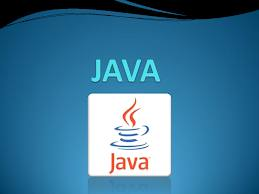
\includegraphics[scale=1]{imagenes/logo.jpeg} 
\caption{Logo Java}
\end{figure}
\end{frame}

\begin{frame}
  \frametitle{Contenido}
  \tableofcontents[pausesections]
\end{frame}



\section{Introduccion}

\begin{frame}
\frametitle{Eventos}\begin{itemize}[<+->]
\item Hasta ahora la interfaces diseñadas no hacen nada, es decir no interactúa con el usuario.
\item Cuando un usuario interáctua con el programa (presiona un botón, introduce un valor en un input, \dots) genera un \emph{evento}.
\item En el programa se diseña \emph{listener (escuchadores)} para realizar lo que el programa debe ejecutar.
\item Un \emph{listener} no es mas que un objeto cuya clase  implementa una derterminada interfaz que está relacionada con un componente de la GUI.
\item El componente que crea el evento se denomina \emph{Objeto fuente o Componente fuente}
\item La clase raíz que gestiona los eventos es \emph{java.util.EventObject}
\end{itemize}
\end{frame}

\begin{frame}
\frametitle{EventObject}
\begin{figure}
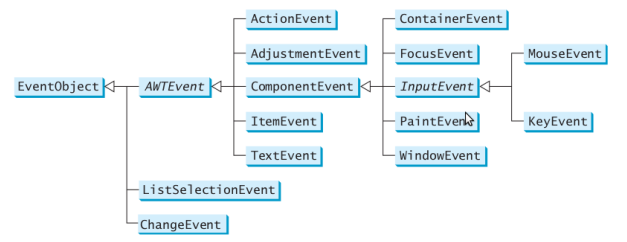
\includegraphics[width=\textwidth]{imagenes/event.png}
\caption{EventObject}
\end{figure}
\end{frame}


\begin{frame}
\frametitle{Acción de usuario, Objeto fuente, Tipo de evento}
\begin{figure}
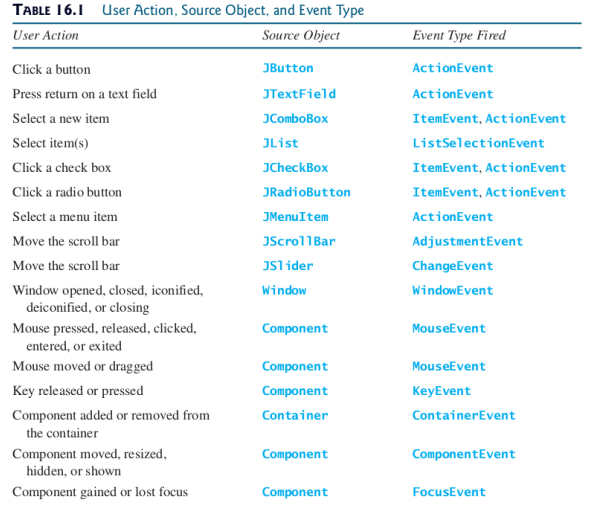
\includegraphics[scale=0.5]{imagenes/uot.png}
%\caption{EventObject}
\end{figure}
\end{frame}

\begin{frame}[fragile]
\frametitle{Listener Object}
\begin{itemize}[<+->]
\item Un \emph{Listener Object} debe tener la correspondiente interfaz para asegurar la gestión adecuada del evento.
\item Generalemente si el evento se denomina \emph{XEvent} la interfaz a implementar es \emph{XListener}.
\item Ejemplo: para \emph{ActionEvent} está \emph{ActionListener}
\item El \emph{Objeto listener} debe ser registrado, dependiendo del tipo de evento.
\item Generalmente para \emph{ActionEvent} tenemos \emph{addActionListener}
\item Ejemplo para \emph{ActionEvent} tenemos el método \emph{addActionListener}
\end{itemize}
\end{frame}

\begin{frame}
\frametitle{Listener}
\begin{figure}
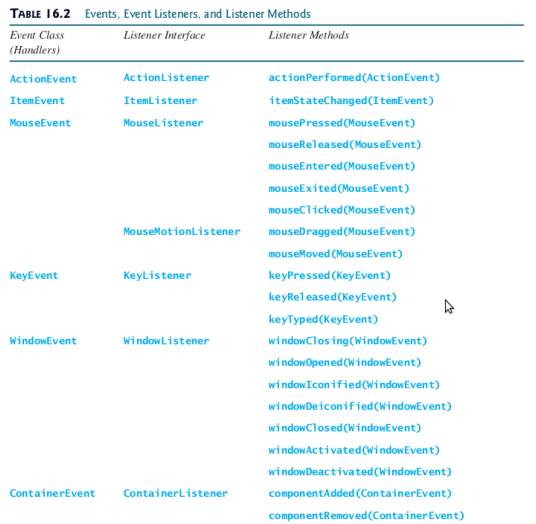
\includegraphics[scale=0.5]{imagenes/listener.png}
%\caption{EventObject}
\end{figure}
\end{frame}

\begin{frame}
\frametitle{Listener} 
\framesubtitle{Ejemplo evento para un botón}
\begin{enumerate}[<+->]
\item Objeto fuente:
\item \emph{JButton jbtOK = new JButton(''OK'');}
\item Objeto listener:
\item \emph{ActionListener listener1 = new OKListenerClass(); }
\item Registramos el listener:
\item \emph{jbtOK.addActionListener(listener1);}
\end{enumerate}
\end{frame}



\begin{frame}[fragile]
    \frametitle{Ejemplo}
\begin{tiny}
\begin{verbatim}
import java.awt.*;
import java.awt.event.*;
import javax.swing.*;

public class DemoListener extends JFrame {
  private JButton boton = new JButton ("Pulsar");
  private JLabel label = new JLabel ();
  public DemoListener (){
    setLayout (new FlowLayout ());
    boton.addActionListener (new PulsarBoton ());
    add (boton);
    add (label);
  }
  
//Clase interna para gestionar el listener
  class PulsarBoton implements ActionListener  {
    public void actionPerformed (ActionEvent e) {
      System.out.println ("Hola");
      label.setText ("Hola");
    }
  }
  
  public static void main (String[]arg) {
    DemoListener frame = new DemoListener ();
    frame.setTitle ("Primer Listener");
    frame.setSize (300, 200);   // Tamaño
    frame.setLocationRelativeTo (null); // Centra
    frame.setDefaultCloseOperation (JFrame.EXIT_ON_CLOSE);      //cierre
    frame.setVisible (true);    // Display la frame
  }
}
\end{verbatim}
\end{tiny}
\end{frame}

\section{Clases internas}
\begin{frame}[fragile]
    \frametitle{Clases internas o anidadas}
 Una clase interna es aquella que está definida dentro del ámbito de otra.
\begin{multicols}{2}
\begin{block}{Clases separadas}
public class Uno \{\\
\dots
\}\\
class Dos\{\\
\dots
\}
\end{block}
\begin{block}{Clases internas}
public class Uno \{\\
\dots\\
class Dos\{\\
\dots
\}\\
\}\\
\end{block}
\end{multicols}
\pause
\begin{itemize}[<+->]
\item En un único archivo sólo puede haber una clase pública.
\item La compilación del primer fichero crea \emph{Uno.class} y \emph{Dos.class}
\item La compilación del segundo archivo crea \emph{Uno.class} y \emph{Uno\$Dos.class}
\end{itemize}
\end{frame}


\begin{frame}
    \frametitle{Clases internas}
\begin{itemize}[<+->]
\item La compilacion de las clases anidadas crea \emph{ClaseExterna\$ClaseInterna.class} como compilacion de la clase anidada o interna.
\item Una clase interna puede referenciar atributos y métodos definidos en las clases externas.
\item Las clases internas pueden estar sujetas a las mismas reglas de visibilidad que los atriubutos y métodos de una clase.
\item Si es creada como pública, se puede acceder desde otro ficheros creando objetos de la clase interna como: \emph{ClaseExterna.ClaseInterna objetoInterno = new ClaseExterna.ClaseInterna()}
\item Una clase interna puede definirse como \emph{static}. Puede usarse de forma que no hace falta crer un objeto de la clase externa. Y no puede referenciar a atributos o métodos \emph{no estáticos}.
\end{itemize}
\end{frame}


\begin{frame}[fragile]
    \frametitle{Clases internas anónimas}
    \begin{multicols}{2}
    \begin{block}{Clase interna}
    public ConstructorClase()\{\\
    \dots\\
    boton.addAdActionListener(\\
    new ControlListener()\\
    \}\\
    class ControlListner()\\
    implements ActionListener\{\\
    public void actionPerFormed\\
    (ActionEvent e)\\
    \{\dots\}\\
    \}
    \end{block}
\begin{block}{Clase interna anonima}
    public ConstrutorClase() \{\\
    \dots\\
    boton.addActionListener(\\
new \st{class ControlListener\\
implements} ActionListener() \{\\
public void actionPerformed\\
(ActionEvent e) \\
\{\\\dots\}\\
\});
\end{block}
\end{multicols}
\pause
La compilación genera las clases \emph{Clase.class} y \emph{Clase\$1.class}
\end{frame}

\subsection{Alternativas al diseño}
\begin{frame}[fragile]
    \frametitle{Alternativas}
  \begin{itemize}[<+->]
  \item Hasta ahora definimos la clase principal como \emph{extends JFrame}
  \item Creamos una clase interna (o interna anónima) que gestiona el evento:
  \item \emph{class PulsarBoton implements ActionListener} por ejemplo.
  \item Pero podemos hacer que la clase principal gestione el evento.
  \item De manera que no hace falta crear una clase interna:
  \item \emph{public class Principal extends JFrame implements ActionListener}
  \item Este diseño implica mucha responsabilidad dentro de una misma clase.
  \item Mejor es diseñar una clase que gestione el \emph{Listener}
  \item El uso de clases internas anónimas o no es un estándar en el diseño de gestión de eventos, por su claridad, limpieza y sencillez del código.
  \end{itemize}
  
\end{frame}

\begin{frame}[fragile]
\frametitle{Ejemplos}
\begin{multicols}{2}
\begin{tiny}
\begin{verbatim}
import javax.swing.*;
import java.awt.event.*;
public class Principal extends JFrame {
// componentes a añadir al frame
 public Principal(){
 //creamos el panel
 //Llamamos al listener
 GestorListener listener = new GestorListener();
 //Registramos listener
 }
 //clase interna
 class GestorListener implements ActionListener{
  public void actionPerformed(ActionEvent e) {
  ......
  }
 }
}
\end{verbatim}
\begin{verbatim}


import javax.swing.*;
import java.awt.event.*;
public class Principal extends JFrame 
 implements ActionListener {
  // componentes a añadir al frame
  public Principal(){
  //creamos el panel
  //registramos listener
  }
  //implementamos el ActionListener
  public void actionPerformed(ActionEvent e) {
   ....
  }
}  
\end{verbatim}
\end{tiny}
\end{multicols}
\end{frame}


\section{Window Event}
\begin{frame}[fragile]
\frametitle{Window Event}
\begin{itemize}[<+->]
\item Hasta ahora hemos usado ActionEvent
\item \emph{WindowEvent} actúa de forma similar.
\item Cualquier subclase de \emph{Window} puede lanzar los siguientes eventos:
\begin{enumerate}
\item window opened
\item window closing
\item window closed
\item window activated
\item window deactivated
\item window iconified
\item window deiconified
\end{enumerate}
\end{itemize}
\end{frame}



\begin{frame}[fragile]
    \frametitle{Ejemplo}
       \begin{tiny}
       \begin{verbatim}
import java.awt.event.*;
import javax.swing.JFrame;
public class TestWindowEvent extends JFrame{
  public static void main (String[]args)  {
    TestWindowEvent frame = new TestWindowEvent ();
      frame.setSize (220, 80);
      frame.setLocationRelativeTo (null);       // Center the frame
      frame.setDefaultCloseOperation (JFrame.EXIT_ON_CLOSE);
      frame.setTitle ("TestWindowEvent");
      frame.setVisible (true);
  }
  public TestWindowEvent ()  {
    addWindowListener (new WindowListener (){
                       public void windowActivated (WindowEvent event){
                         System.out.println ("Window activated");}
                       public void windowDeiconified (WindowEvent event){
                         System.out.println ("Window deiconified");}
                       public void windowIconified (WindowEvent event){
                         System.out.println ("Window iconified");}
                       public void windowDeactivated (WindowEvent event){
                         System.out.println ("Window deactivated");}
                       public void windowOpened (WindowEvent event){
                         System.out.println ("Window opened");}
                       public void windowClosing (WindowEvent event){
                         System.out.println ("Window closing");}
                       public void windowClosed (WindowEvent event){
                         System.out.println ("Window closed");}
                       });
  }
       \end{verbatim}
       \end{tiny}
       Hay que implementar todos los métodos para que funcione.
\end{frame}

\begin{frame}[fragile]
\frametitle{Clases Adapter}
\begin{itemize}[<+->]
\item Los métodos de la interfaz \emph{WindowListener} son abstractos.
\item Cuando los métodos son abstractos, implica que hay implementarlos.
\item En el caso de \emph{WindowListener} hay que implementar \emph{windowActivated, windowDeiconified, \dots}. \emph{TODOS}
\item Java provee clases denominadas \emph{convenience adapters} que conlleva implementaciones por defecto.
\end{itemize}
\pause
\begin{figure}
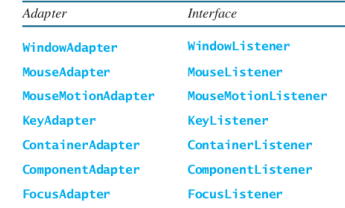
\includegraphics[scale=0.5]{imagenes/adapter.png}
\end{figure}
\end{frame}


\begin{frame}[fragile]
    \frametitle{Ejemplo}
\begin{footnotesize}
\begin{verbatim}
import java.awt.event.*;
import javax.swing.JFrame;
public class AdapterDemo extends JFrame
{
  public static void main (String[]args)
  {
    AdapterDemo frame = new AdapterDemo ();
      frame.setSize (220, 80);
      frame.setLocationRelativeTo (null);       // Center the frame
      frame.setDefaultCloseOperation (JFrame.EXIT_ON_CLOSE);
      frame.setTitle ("AdapterDemo");
      frame.setVisible (true);
  }
  public AdapterDemo () {
    addWindowListener (new WindowAdapter (){
                       public void windowActivated (WindowEvent event)
                       {
                       System.out.println ("Window activated");}
                       });
  }
}
\end{verbatim}
\end{footnotesize}
\end{frame}


\section{Eventos de raton}
\subsection{interfaz MouseListener}
\begin{frame}[fragile]
\frametitle{MouseListener}
\framesubtitle{Metodos de la interfaz MouseListener}
\begin{description}
\item[public  void mousePressed(MouseEvent evento)] Es llamado cuando se oprime un botón en el Mouse.
\item[public  void mouseClicked(MouseEvent evento)] Se llama cuando se oprime y se suelta un botón en el mouse.
\item[public  void mouseReleased(MouseEvent evento)] Ocurre cuando se suelta un botón en el Mouse.
\item[public  void mouseEntered(MouseEvent evento)] Ocurre cuando el cursor entra dentro de los límites del componente.
\item[public  void mouseExited(MouseEvent evento)] Ocurre cuando el cursor sale dentro de los límites del componente.               
\end{description}
\end{frame}

\subsection*{interfaz  MouseMontionListener}
\begin{frame}[fragile]
\frametitle{ MouseMontionListener}
\framesubtitle{Metodos de la interfaz  MouseMontionListener}
\begin{description}
\item[public  void mouseDragged(MouseEvent evento)] ocurre cuando el boton del raton se oprime mientras el cursor esta sobre un componente y se mueve mientras se mantiene presionado.
\item[public  void mouseMoved(MouseEvent evento)] Ocurre al moverse el raton cuando se encuentra sobre un componente.
\item[mouseWheelMoved(MouseWheelEvent e)] La clase MouseWheelEvent es una subclase de MouseEvent y contiene los métodos que permiten al manejador de eventos obtener la información necesaria acerca de la rotación de la rueda giratoria.
\end{description}
\end{frame}


\subsection{MouseEvent}
\begin{frame}
\frametitle{java.awt.MouseEvent.*}
\begin{figure}
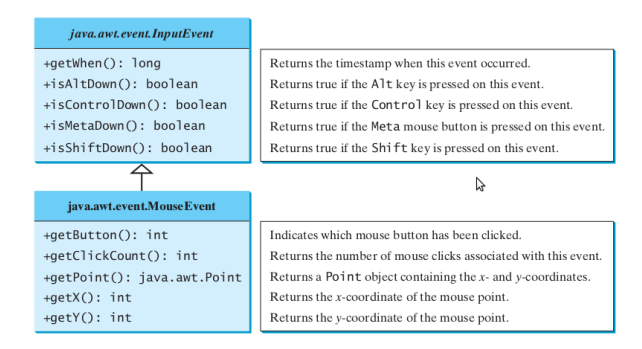
\includegraphics[width=\textwidth]{imagenes/mousevent.png}
\end{figure}
\end{frame}

\begin{frame}[fragile]
\frametitle{Ejemplo} 
\begin{tiny}
\begin{verbatim}
import java.awt.*;
import java.awt.event.*;
public class MouseClick{
  Label lbl;
  public static void main (String[]args)  {
    MouseClick MC = new MouseClick ();
  }
  public MouseClick ()  {
    Frame f = new Frame ("Checking the mouse click");
    Panel p = new Panel ();
    Button button = new Button ("Click Me");
    button.addMouseListener (new MyMouseListener ());
    p.add (button, BorderLayout.NORTH);
    f.add (p, BorderLayout.NORTH);
    lbl = new Label ("Roseindia.net");
    f.add (lbl, BorderLayout.CENTER);
    f.addWindowListener (new WindowAdapter (){
                         public void windowClosing (WindowEvent we){
                         System.exit (0);
                         }});
    f.setSize (400, 400);
    f.setVisible (true);
  }
public class MyMouseListener extends MouseAdapter  {
    public void mouseClicked (MouseEvent me){
      String str = lbl.getText ();
      if (str.equals ("Roseindia.net")) {
          lbl.setText ("You have clicke the button.");
        }
      else if (str.equals ("You have clicke the button.")){
          lbl.setText ("Roseindia.net");
        }
    }
  }
}
\end{verbatim}
\end{tiny}
\end{frame}

\section{Eventos de teclado}
\begin{frame}[fragile]
\frametitle{Eventos de teclado}
\begin{itemize}[<+->]
\item Se produce cuando pulsamos una tecla, soltamos una tecla o bien introducimos datos por teclado.
\item \emph{Objetos KeyEvent} describen la naturaleza del evento.
\item \emph{Interfaz KeyListener} manejan los eventos de teclado.
\end{itemize}
\pause
\begin{block}{java.awt.event.InputEvent}
+getKeyChar(): char \emph{devuelve el caracter asociado a la tecla}\\
+getKeyCode(): int \emph{Devuelve el código asociada a dicha tecla}
\end{block}
\pause
\begin{block}{java.awt.event.KeyListener}
+keyPressed(e: KeyEvent): void \emph{se invoca después de presionar una tecla}\\
+keyReleased(e: KeyEvent): void \emph{se invoca después de soltar una tecla}\\
+keyTyped(e: KeyEvent): void \emph{e invoca después de presionar y soltar una tecla}
\end{block}
\end{frame}

\begin{frame}
\frametitle{Preguntas} 
\begin{figure}

\includegraphics[scale=0.9]{imagenes/dudas.png} 
\end{figure} 
\end{frame}

\end{document}

